\documentclass[tikz,border=4pt]{standalone}
% Shared style for MultiMM figures (white background, logo palette)
\usepackage{tikz,pgfplots,amsmath}
\pgfplotsset{compat=1.16}
\usetikzlibrary{arrows.meta,calc,decorations.pathreplacing,positioning,backgrounds}
\definecolor{indigo}{HTML}{3B37A0}
\definecolor{violet}{HTML}{6A3AA8}
\definecolor{crimson}{HTML}{B5406C}
\definecolor{gold}{HTML}{E9A62C}
\definecolor{golddark}{HTML}{B9791A}
\definecolor{grey}{HTML}{8A8AA0}
\definecolor{lightgrey}{HTML}{E4E4EE}
\tikzset{
  bead/.style={circle,draw=#1!80!black,fill=#1!35,line width=0.5pt,minimum size=9pt,inner sep=0pt},
  bead/.default=indigo,
  lab/.style={font=\small},
}
\pgfplotsset{
  every axis/.append style={
    width=9.5cm,height=6.3cm,axis lines=left,line width=0.5pt,
    grid=major,grid style={draw=lightgrey,line width=0.3pt},
    tick label style={font=\small},label style={font=\normalsize},
    legend style={font=\footnotesize,draw=none,fill=white,fill opacity=0.8,text opacity=1},
    legend cell align=left,
  },
  every axis plot/.append style={line width=1.2pt,smooth},
}

\begin{document}
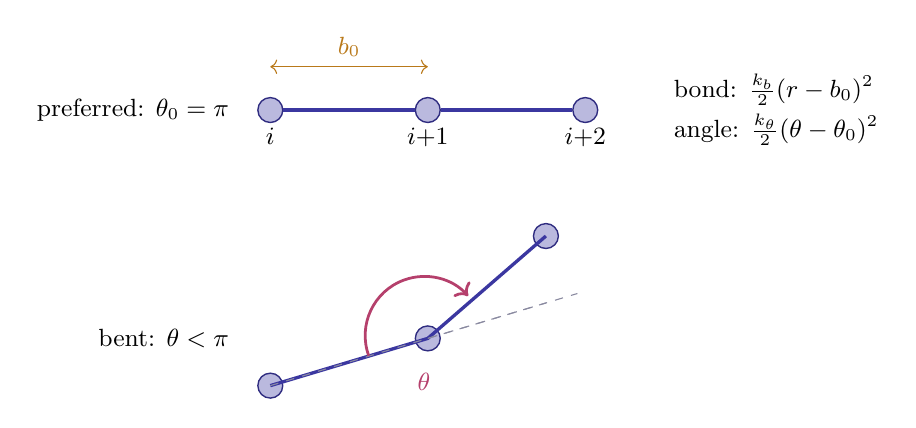
\begin{tikzpicture}
% left: straight chain, theta = pi
\node[lab,anchor=east] at (-0.4,0.9) {preferred: $\theta_0=\pi$};
\foreach \x/\n in {0/i,2/i{+}1,4/i{+}2}{\node[bead] (b\x) at (\x,0.9) {};
  \node[lab,below=3pt] at (b\x) {$\n$};}
\draw[line width=1.2pt,indigo] (b0)--(b2)--(b4);
\draw[<->,golddark] (0,1.45)--(2,1.45) node[midway,above,lab] {$b_0$};
% right: bent chain
\begin{scope}[shift={(0,-2.6)}]
\node[lab,anchor=east] at (-0.4,0.6) {bent: $\theta<\pi$};
\coordinate (p0) at (0,0); \coordinate (p1) at (2,0.6); \coordinate (p2) at (3.5,1.9);
\foreach \p/\n in {p0/i,p1/i{+}1,p2/i{+}2}{\node[bead] at (\p) {}; }
\draw[line width=1.2pt,indigo] (p0)--(p1)--(p2);
\draw[dashed,grey] (p0)--($(p1)!-0.75!(p0)$)  ;
\draw[dashed,grey] (p1)--($(p1)!1.0!(p1)+(1.9,0.57)$);
\draw[crimson,line width=1pt,->] ($(p1)+(-0.75,-0.22)$) arc (200:42:0.75);
\node[crimson,lab] at ($(p1)+(0.1,0.0)+(-0.15,-0.55)$) {$\theta$};
\end{scope}
\node[lab,align=left,anchor=west] at (5,0.9) {bond: $\tfrac{k_b}{2}(r-b_0)^2$\\[2pt]angle: $\tfrac{k_\theta}{2}(\theta-\theta_0)^2$};
\end{tikzpicture}
\end{document}
